|\chapter{MARCO TEÓRICO}

En el presente capítulo se presentan los conceptos teóricos necesarios para abordar el diseño e implementación de un sistema de monitoreo y alerta en tiempo real de niveles de CO2 en aulas empleando comunicación inalámbrica LoRa en una red IoT.

\section{Protocolo LoRa}
LoRa (Long Range) es una tecnología de comunicación inalámbrica diseñada para redes IoT que requieren comunicaciones a largas distancias con un bajo consumo de energía. Su principal ventaja es su capacidad para transmitir datos a distancias que pueden alcanzar los 15 km en áreas rurales y entre 1-3 km en entornos urbanos densos. LoRa opera en bandas de frecuencia ISM no licenciadas, como 433 MHz, 868 MHz (Europa) y 915 MHz (Norteamérica). Su éxito se debe al uso de la modulación Chirp Spread Spectrum (CSS), que codifica la información a través de chirps de frecuencia, permitiendo que LoRa resista interferencias y mantenga la estabilidad de la señal en entornos desafiantes, con una sensibilidad del receptor que puede alcanzar -130 dBm \cite{A_Study_of_LoRa_Long_Range_and_Low_Power_Networks_for_the_Internet_of_Things}.

El rendimiento de LoRa depende de tres parámetros clave: el Spreading Factor (SF), el ancho de banda (BW) y la tasa de corrección de errores (CR). El SF, que varía entre 7 y 12, permite ajustar la relación entre la distancia de transmisión y la tasa de datos. Un SF más alto aumenta el alcance de la señal pero disminuye la velocidad de transmisión. La tasa de símbolos (Rs) se calcula con la fórmula:

\begin{equation}\label{eq
	} Rs = \frac{SF \cdot BW}{2^{SF}} \end{equation}

Por otro lado, la tasa de datos (Rb) también depende del SF y el BW, y se puede calcular con:

\begin{equation}\label{eq
	} Rb = \frac{SF \cdot \left( \frac{4}{4+CR} \right) \cdot BW}{2^{SF}} \cdot 1000 \end{equation}

Dependiendo de la configuración de estos parámetros, LoRa puede ajustarse para optimizar la cobertura o la tasa de bits, según la aplicación IoT específica \cite{A_Survey_of_LoRaWAN_for_IoT_From_Technology_to_Application}.


\section{Red LoRaWAN}
LoRaWAN es el protocolo de red que se utiliza sobre la capa física de LoRa para gestionar las comunicaciones entre los dispositivos IoT y los servidores de red. LoRaWAN sigue una topología de estrella, donde los dispositivos finales envían datos a través de gateways, que los retransmiten a un servidor de red central. Existen tres clases de dispositivos en LoRaWAN, cada uno diseñado para distintos escenarios de consumo energético \cite{A_Study_of_LoRa_Long_Range_and_Low_Power_Networks_for_the_Internet_of_Things} \cite{A_Survey_of_LoRaWAN_for_IoT_From_Technology_to_Application}:

\begin{itemize}
	\item \textbf{Clase A}: Optimiza el consumo energético al permitir dos ventanas de recepción cortas después de cada transmisión.
	\item \textbf{Clase B}: Añade ventanas de recepción programadas, permitiendo una mayor flexibilidad.
	\item \textbf{Clase C}: Mantiene las ventanas de recepción abiertas casi todo el tiempo, lo que mejora la capacidad de respuesta pero incrementa el consumo energético.
\end{itemize}
LoRaWAN también incluye el mecanismo de ratio de data adaptativo (ADR: adaptive data rate), que ajusta dinámicamente el SF y la potencia de transmisión para maximizar la eficiencia energética y la fiabilidad de la comunicación.

%En términos de rendimiento, LoRaWAN es sensible a la carga de la red. En simulaciones con 500,000 paquetes, se encontró que la capacidad máxima del canal era del 18\%, y las colisiones aumentaron al 60\% cuando la carga alcanzó el 48\%, lo que limita su escalabilidad en entornos con alta densidad de dispositivos IoT (fuente 1 y fuente 2).

\begin{figure}[H]
	\centering
	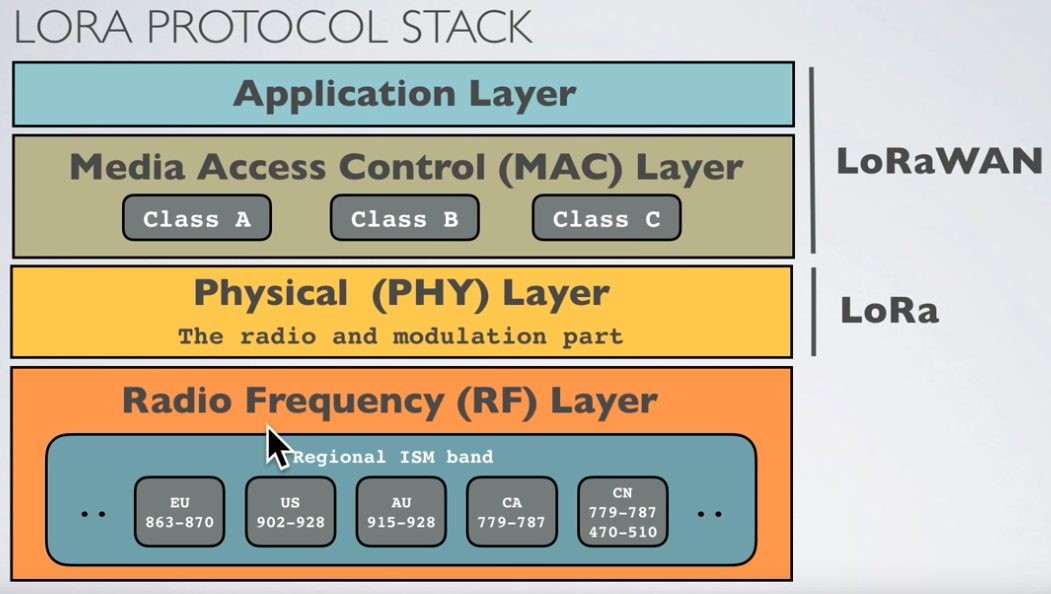
\includegraphics[width=1\linewidth]{images/capitulo2/lora_stack.png}
	\caption{\centering Pila de protocolo LoRa \cite{lora_stack}.}
	\label{fig:lora_stack}
\end{figure}

La pila del protocolo LoRa , tal y como se muestra en la Figura \ref{fig:lora_stack} se divide en varias capas. En la base se encuentra la capa de frecuencia de radio (RF), que define las bandas regionales ISM utilizadas para la transmisión (como las bandas de 863-870 MHz en Europa y 902-928 MHz en EE.UU.). Encima está la capa física (PHY), que se encarga de la radio y la modulación de la señal. La capa de control de acceso al medio (MAC) incluye las clases A, B y C, que definen diferentes modos de transmisión y recepción, ajustando el consumo de energía. En la parte superior está la capa de aplicación, que interactúa directamente con los servicios y aplicaciones de los usuarios. LoRaWAN abarca la capa MAC y la capa de aplicación.

\begin{figure}[H]
	\centering
	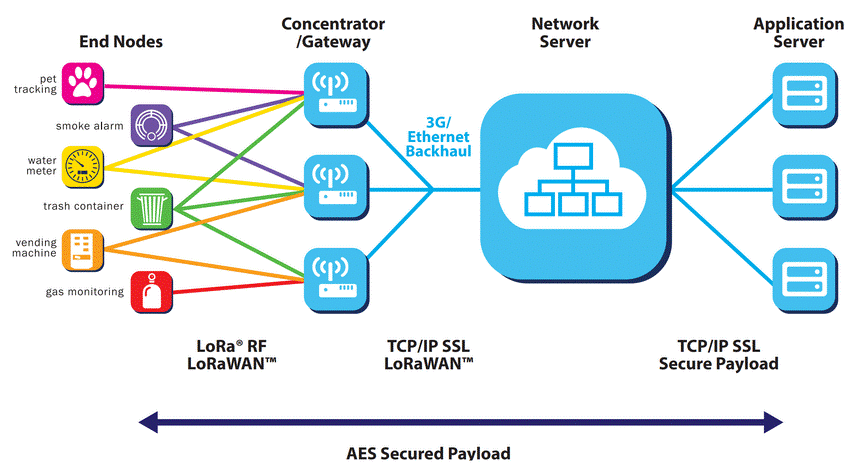
\includegraphics[width=1\linewidth]{images/capitulo2/lora_arq.png}
	\caption{\centering Arquitectura de una red LoRaWAN enfocada en nodos finales múltiples \cite{lora_alliance}.}
	\label{fig:lora_arq}
\end{figure}

\begin{figure}[H]
	\centering
	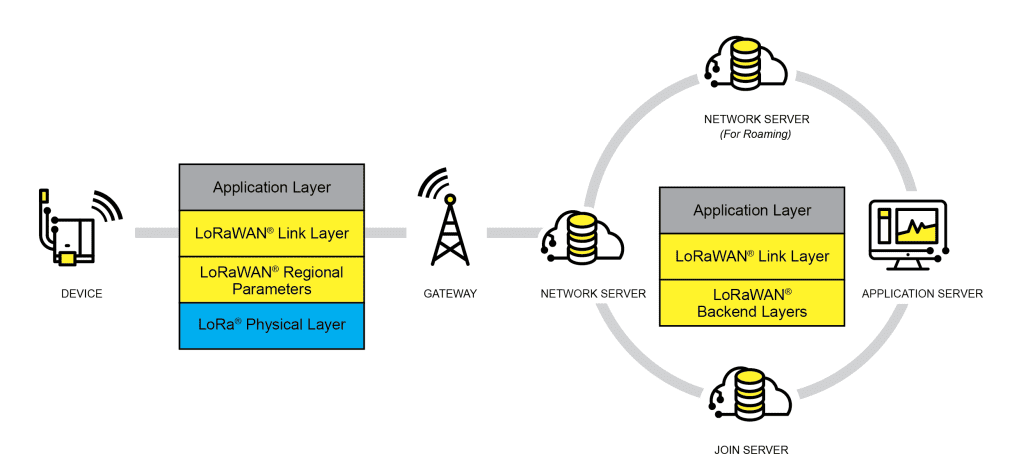
\includegraphics[width=1\linewidth]{images/capitulo2/lorawan_arq.png}
	\caption{\centering Arquitectura de una red LoraWAN enfocada en servidores múltiples \cite{lora_alliance}.}
	\label{fig:lorawan_arq}
\end{figure}

El funcionamiento de LoRaWAN en una red de dispositivos conectados como se muestra en la Figuras \ref{fig:lora_arq} y \ref{fig:lorawan_arq}. Un dispositivo envía datos a través de una gateway, que luego los transmite a un servidor de red. El servidor de red, a su vez, se comunica con los servidores de aplicaciones y servidores de registro (join server), que gestionan el acceso y almacenamiento de los datos. La imagen destaca cómo las capas del protocolo (física, parámetros regionales, y de enlace) se usan para garantizar la comunicación eficiente entre los diferentes elementos de la red.

\section{Descripción de componentes utilizados para el nodo sensor de CO\(_2\)}

A continuación se muestran los componentes electrónicos requeridos para un nodo sensor o nodo final (end node), tal y como se muestra en la Figura \ref{fig: estructura_general_IoT}. Estos nodos recopilan información de su entorno mediante sensores, tranmitirla o recibir instrucciones del gateway, por lo que mantienen una comunicación bidireccional.

\begin{figure}[H]
	\centering
	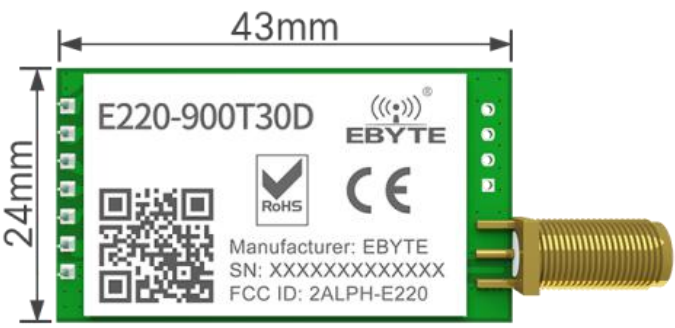
\includegraphics[width=0.65\linewidth]{images/capitulo2/modulo_lora.png}
	\caption{\centering Módulo LoRa E220-900T30D \cite{modulo_lora}.}
	\label{fig:modulo_lora}
\end{figure}

El módulo E220-900T30D, mostrado en la Figura \ref{fig:modulo_lora}, es un dispositivo que utiliza tecnología LoRa para comunicación en la banda de 868/915 MHz, basado en el chip LLCC68. Ofrece una transmisión eficiente a largas distancias, alcanzando hasta 10 km en condiciones óptimas, y presenta una alta capacidad de resistencia a interferencias. Admite diferentes modos de operación, incluyendo transmisión fija y por difusión, además de contar con funciones de monitoreo y activación por aire, lo que lo hace ideal para aplicaciones que requieren bajo consumo de energía. Este módulo puede funcionar con voltajes de 3.0 a 5.5V, siendo compatible con niveles de 3.3V y 5V en sus interfaces UART. Con un consumo mínimo en modo de suspensión (alrededor de 5 $\mu$A), es adecuado para aplicaciones como automatización del hogar, sistemas de seguridad y control remoto en entornos industriales, soportando temperaturas extremas de $-40$ a $+85$ °C.



\begin{figure}[H]
	\centering
	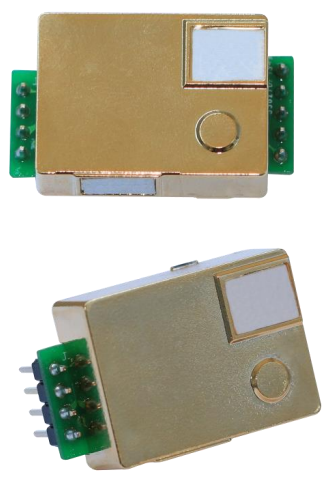
\includegraphics[width=0.65\linewidth]{images/capitulo2/sensor_co2.png}
	\caption{\centering Sensor de CO\(_2\) MH-Z19B \cite{sensor_co2}.}
	\label{fig:sensor_co2}
\end{figure}

El sensor MH-Z19B es un módulo infrarrojo no dispersivo (NDIR: non dispersive infrared detector) que permite detectar CO\(_2\) en el aire de manera precisa y estable. Su diseño compacto y de bajo consumo incluye compensación de temperatura, lo que lo hace adecuado para aplicaciones como la monitorización de calidad del aire en interiores, sistemas de climatización (HVAC: heating, ventilation and air conditioning) y dispositivos inteligentes. Ofrece múltiples opciones de salida de datos, incluyendo UART y PWM, y es capaz de medir concentraciones de CO\(_2\) en un rango de 0 a 2000 ppm o hasta 5000 ppm, con un tiempo de respuesta inferior a 120 segundos y una vida útil superior a los 5 años.




\begin{figure}[H]
	\centering
	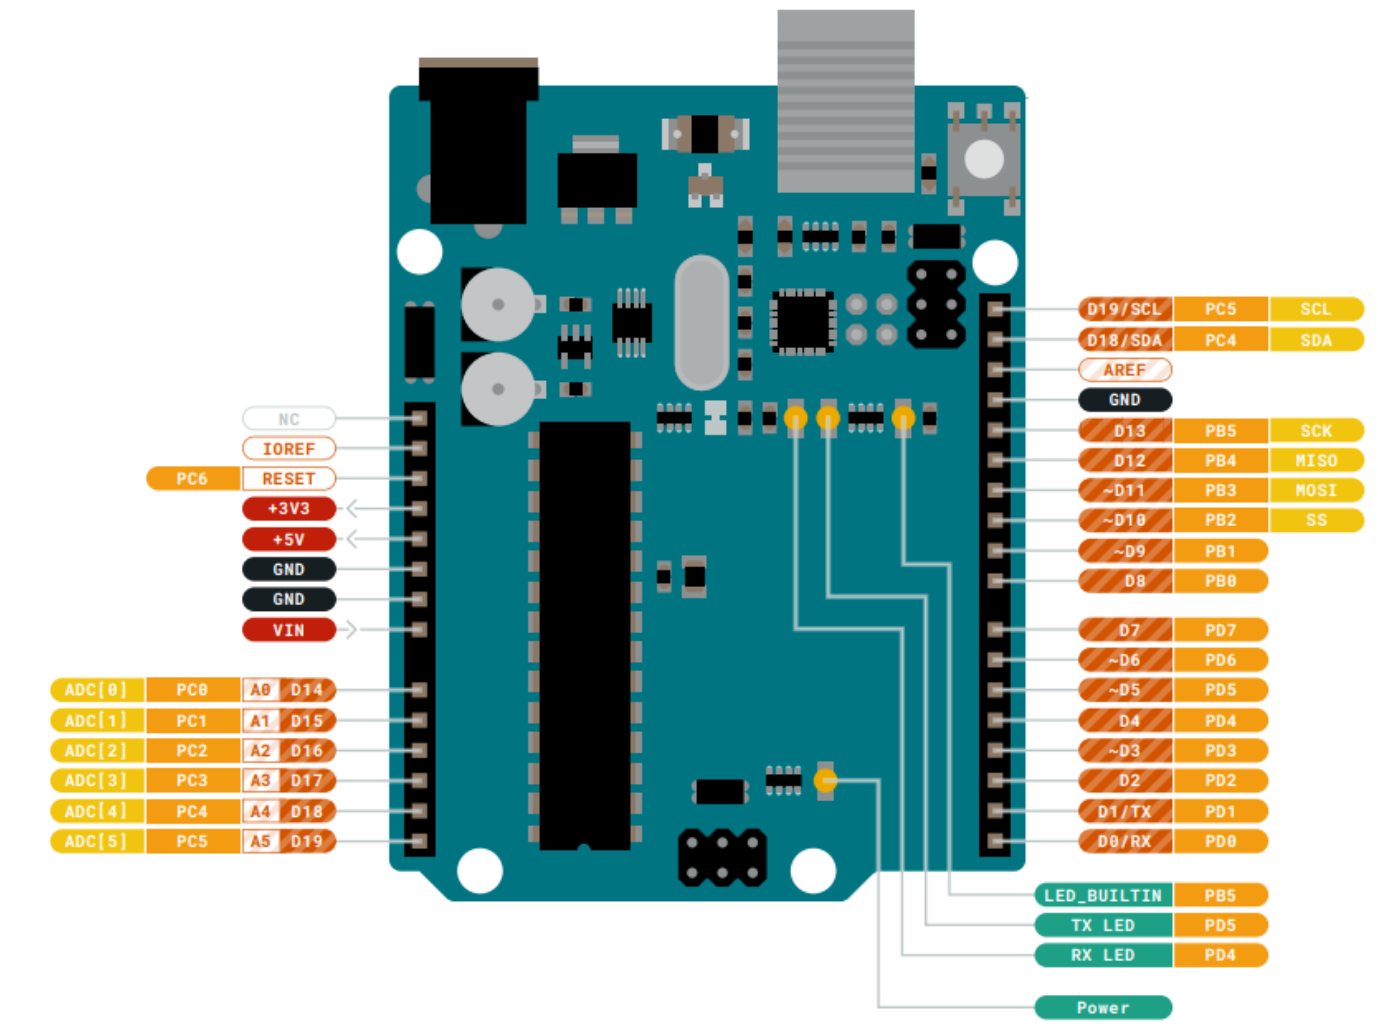
\includegraphics[width=0.65\linewidth]{images/capitulo2/arduino_uno_pins_datasheet.png}
	\caption{\centering Sensor de CO\(_2\) \cite{arduino_uno_datasheet}.}
	\label{fig:arduino}
\end{figure}

El microcontrolador ATMEGA328P, el cual es utilizado en la placa Arduino UNO mostrada en la Figura \ref{fig:arduino}, está basado en una arquitectura AVR de 8 bits y opera a una frecuencia máxima de 16 MHz. Ofrece una memoria Flash de 32 KB, 2 KB de SRAM y 1 KB de EEPROM, junto con múltiples interfaces de comunicación, como UART, SPI e I2C. Además, cuenta con un convertidor ADC de 10 bits y varios temporizadores, lo que lo hace adecuado para aplicaciones de control y monitoreo. Funciona en un rango de voltaje de 1.8 a 5.5 V y admite modos de bajo consumo, como Power-save, Standby y Power-down, lo que lo convierte en una excelente opción para proyectos de electrónica educativa y aplicaciones embebidas que no requieren altas velocidades de procesamiento \cite{arduino_uno_datasheet}.








\section{Amazon Web Services (AWS)}
Amazon Web Services (AWS) es una plataforma de computación en la nube proporcionada por Amazon, que ofrece una extensa variedad de servicios bajo demanda, como almacenamiento, bases de datos, capacidad de cómputo y soluciones de redes. Funciona a través de una infraestructura global de centros de datos, lo que permite a los usuarios acceder a recursos de manera flexible y pagar un monto variable en función a los recursos utilizados. AWS facilita a empresas y desarrolladores el despliegue y escalado rápido de aplicaciones sin la necesidad de invertir en infraestructura física. Se emplea principalmente para alojar aplicaciones web, manejar grandes volúmenes de datos y ejecutar análisis en tiempo real, ayudando a optimizar costos y recursos operativos.


\section{SQL Server Management Studio}
SQL Server Management Studio (SSMS) es una herramienta de administración para trabajar con instancias de bases de datos SQL Server, tanto en instalaciones locales como en la nube. Permite gestionar servidores y bases de datos mediante una interfaz gráfica intuitiva, facilitando la creación de consultas, gestión de objetos de base de datos, monitoreo de rendimiento y ejecución de scripts. Funciona integrando herramientas avanzadas para desarrolladores y administradores de bases de datos, simplificando tareas como la configuración de servidores, monitoreo y análisis de consultas \cite{sql_server}.



\section{.NET Core}
.NET es una plataforma de desarrollo multiplataforma y de código abierto que permite crear aplicaciones en una variedad de lenguajes, como C\# y Visual Basic. Funciona ofreciendo un entorno de ejecución eficiente, herramientas avanzadas, y un conjunto de bibliotecas para crear aplicaciones de escritorio, móviles, web y servicios en la nube. .NET permite a los desarrolladores construir soluciones escalables y de alto rendimiento, tanto para entornos locales como en la nube, y es ideal para proyectos modernos que requieren flexibilidad y compatibilidad multiplataforma \cite{net_core}.





